\documentclass{beamer}

\usepackage{color}
\definecolor{greenish}{RGB}{152,204,112}
\definecolor{redish}{RGB}{244,158,196}


\setbeamertemplate{navigation symbols}{}
\usepackage{beamerthemeshadow}

\newcommand*{\LargerCdot}{\raisebox{-0.25ex}{\scalebox{3.0}{$\cdot$}}}

\usepackage{mathrsfs}

% \expandafter\def\expandafter\insertshorttitle\expandafter{%
%   \insertshorttitle\hfill%
%   \insertframenumber\,/\,\inserttotalframenumber}

\expandafter\def\expandafter\insertshorttitle\expandafter{%
  \insertshorttitle\hfill%
  \insertframenumber}


\begin{document}

\title{Active Learning}  
\author{Kacper Sokol}
\date{\today} 
\begin{frame}
\titlepage
\end{frame}




\begin{frame}
  \frametitle{Table of contents}
  \tableofcontents
\end{frame} 


\section{Concept of learning} 
  \subsection{Clustering}
  \begin{frame}%[plain]
    \frametitle{Find two clusters} 
    \begin{figure}
      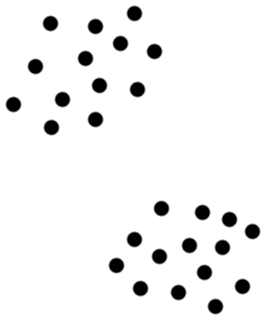
\includegraphics[scale=.5]{graphics/presentation/clusters1} 
    \end{figure}
  \end{frame}

  \begin{frame}%[plain]
    \frametitle{Find two clusters cont.} 
    \begin{figure}
      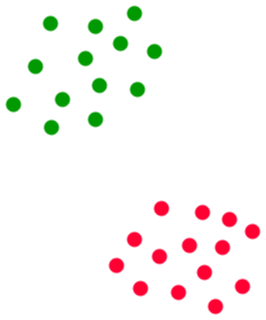
\includegraphics[scale=.5]{graphics/presentation/clusters1a} 
    \end{figure}
  \end{frame}

  \begin{frame}%[plain]
    \frametitle{Find two clusters cont.} 
    \begin{figure}
      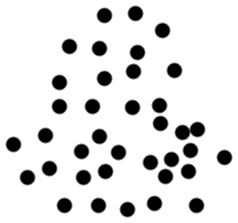
\includegraphics[scale=.5]{graphics/presentation/clusters2} 
    \end{figure}
  \end{frame}

  \begin{frame}%[plain]
    \frametitle{Find two clusters cont.} 
    \begin{figure}
      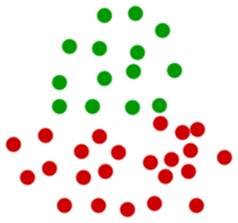
\includegraphics[scale=.5]{graphics/presentation/clusters2a} 
    \end{figure}
  \end{frame}

  \begin{frame}%[plain]
    \frametitle{Find two clusters cont.} 
    \begin{figure}
      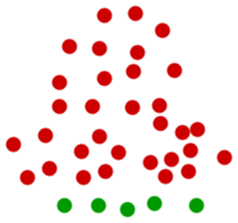
\includegraphics[scale=.5]{graphics/presentation/clusters2b} 
    \end{figure}
  \end{frame}

  \begin{frame}%[plain]
    \frametitle{Find two clusters cont.} 
    \begin{figure}
      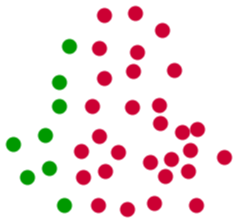
\includegraphics[scale=.5]{graphics/presentation/clusters2c} 
    \end{figure}
  \end{frame}

  \begin{frame}%[plain]
    \frametitle{Find two clusters cont.} 
    \begin{figure}
      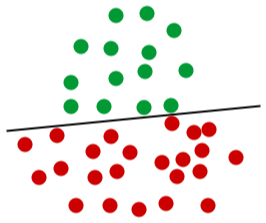
\includegraphics[scale=.5]{graphics/presentation/clusters2d} 
    \end{figure}
  \end{frame}

\subsection{The task}
  \begin{frame}
    \frametitle{Linear classifier}
    \begin{columns}
      \begin{column}{5cm}
        \begin{itemize}
          \item We are handling \textbf{binary classification}.
          \item The data are \textbf{linearly separable}.
          \item Therefore, our goal is to find two clouds of points separated by a straight line and make no error in separation.
        \end{itemize}
      \end{column}
      \begin{column}{5cm}
        \begin{figure}
          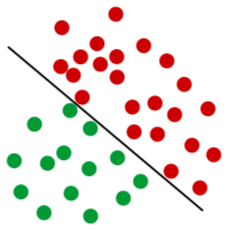
\includegraphics[scale=.4]{graphics/presentation/clusters2e} 
        \end{figure}
        \begin{itemize}
          \item green---a bike; red---a car
          \item x-axis---age of a person
          \item y-axis---distance form home to office/school
        \end{itemize}
      \end{column}
    \end{columns}
  \end{frame}

  \begin{frame}
    \frametitle{Linear classifier}
    \begin{block}{Theory of linear classifier}
      A linear classifier can be defined by a single vector $\mathbf{w} \in \mathbb{R}^N$, where dimension $N$ corresponds to number of parameters characterising our data---in this particular case $N=2$.
      $$
        \text{class}(\mathbf{x}) = \mathbf{w} \cdot \mathbf{x} - t \text{  ,  } \mathbf{x} \rightarrow \begin{cases} \textcolor{redish}{\LargerCdot} \text{ or } \textcolor{redish}{+} & \text{class}(\mathbf{x}) > 0 \\ \textcolor{greenish}{\LargerCdot} \text{ or } \textcolor{greenish}{-} & \text{class}(\mathbf{x}) < 0  \end{cases}
      $$
      In the above equation $t$ is arbitrarily chosen threshold.
    \end{block}
  \end{frame}

  \begin{frame}
    \frametitle{Linear classifier, cont.}
    \begin{block}{Evaluating the classifier---loss function}
      % ---is a value calculated for a given data points which
      \textit{Loss} describes how well given classifier fits the data; loss is positive if a point is classified correctly(the higher, the better), and it is negative if a point is classified incorrectly(the lower, the worse).\\
      Exponential loss:
      $$
        L_{\text{exp}}(z) = \exp(-z) \text{  ,  } z(\mathbf{x}) = \text{label}(\mathbf{x}) * \text{class}(\mathbf{x}) \text{ ,}
      $$
      where $\text{label}(\mathbf{x})$ is the \textbf{true class} of datum point $\mathbf{x}$ i.e.\ $\textcolor{red}{+}$ or $\textcolor{green}{-}$.
    \end{block}
  \end{frame}

  \begin{frame}
    \frametitle{Supervised learning, cont.}
    In supervised learning we are given \emph{data points} together with their \emph{true class} and use this information to learn \emph{weight vector} $\mathbf{w}$.
    \begin{columns}
      \begin{column}{3cm}
        \begin{block}{Dataset---Spam}
          \begin{align*}
            (1,5)  & \rightarrow \textcolor{green}{\LargerCdot}\\
            (0,7)  & \rightarrow \textcolor{green}{\LargerCdot}\\
            (2,9)  & \rightarrow \textcolor{green}{\LargerCdot}\\
            (12,0) & \rightarrow \textcolor{red}{\LargerCdot}\\
            (8,3)  & \rightarrow \textcolor{red}{\LargerCdot}\\
            (13,1) & \rightarrow \textcolor{red}{\LargerCdot}
          \end{align*}
        \end{block}
      \end{column}
      \begin{column}{3cm}
        \begin{block}{Learn parameters}
          Use learning algorithm to learn weight vector $\mathbf{w}$ and class threshold $t$.\\
          ~\vspace*{.45cm}
          $$
            \mathbf{w} = (5,1)
          $$
          $$
            t = 33
          $$
        \end{block}
      \end{column}
      \begin{column}{3cm}
        \begin{block}{Classification}
          \begin{align*}
            -23 <0  & \rightarrow \textcolor{greenish}{\LargerCdot}\\
            -26  <0 & \rightarrow \textcolor{greenish}{\LargerCdot}\\
            -14  <0 & \rightarrow \textcolor{greenish}{\LargerCdot}\\
            27 >0 & \rightarrow \textcolor{redish}{\LargerCdot}\\
            10  >0 & \rightarrow \textcolor{redish}{\LargerCdot}\\
            33 >0 & \rightarrow \textcolor{redish}{\LargerCdot}
          \end{align*}
        \end{block}
      \end{column}
    \end{columns}
  \end{frame}

  \begin{frame}
    \frametitle{Supervised learning}
    Overall loss:
    \begin{multline*}
      \exp(-(\textcolor{green}{-} * -23)) + \exp(-(\textcolor{green}{-} * -26)) + \exp(-(\textcolor{green}{-} * -14)) +\\ \exp(-(\textcolor{red}{+} * 27)) + \exp(-(\textcolor{red}{+} * 10)) + \exp(-(\textcolor{red}{+} * 33)) =\\ 0.0000462315680937 \text{ .}
    \end{multline*}
    For comparison, with one mistake on datum point $(13,1)$ we would get the loss of $214,643,579,786,000$.
    \begin{columns}
      \begin{column}{5cm}
        \begin{block}{Dataset---Spam}
          \begin{align*}
            (1,5)  & \rightarrow \textcolor{green}{\LargerCdot} \text{~~~~} (12,0) & \rightarrow \textcolor{red}{\LargerCdot}\\
            (0,7)  & \rightarrow \textcolor{green}{\LargerCdot} \text{~~~~} (8,3)  & \rightarrow \textcolor{red}{\LargerCdot}\\
            (2,9)  & \rightarrow \textcolor{green}{\LargerCdot} \text{~~~~} (13,1) & \rightarrow \textcolor{red}{\LargerCdot}
          \end{align*}
        \end{block}
      \end{column}
      \begin{column}{5cm}
        \begin{block}{Classification}
          \begin{align*}
            -23 <0  & \rightarrow \textcolor{greenish}{\LargerCdot} \text{~~~} 27 >0 & \rightarrow \textcolor{redish}{\LargerCdot}\\
            -26  <0 & \rightarrow \textcolor{greenish}{\LargerCdot} \text{~~~} 10  >0 & \rightarrow \textcolor{redish}{\LargerCdot}\\
            -14  <0 & \rightarrow \textcolor{greenish}{\LargerCdot} \text{~~~} 33 >0 & \rightarrow \textcolor{redish}{\LargerCdot}
          \end{align*}
        \end{block}
      \end{column}
    \end{columns}
  \end{frame}

\subsection{Active learning}
  \begin{frame}
    \frametitle{Active learning}
    \begin{block}{Dataset}
      \begin{align*}
        (1,5)  & \rightarrow \textcolor{black}{\LargerCdot} \text{~~~~} (0,7)  \rightarrow \textcolor{black}{\LargerCdot} \text{~~~~} (2,9)  \text{~} \rightarrow \textcolor{black}{\LargerCdot}\\
        (12,0) & \rightarrow \textcolor{black}{\LargerCdot} \text{~~~~} (8,3)  \rightarrow \textcolor{black}{\LargerCdot} \text{~~~~} (13,1)  \rightarrow \textcolor{black}{\LargerCdot}
      \end{align*}
    \end{block}
    \begin{itemize}
      \item We are provided data without \textbf{ground truth}...
      \item ...but, we have access to \textbf{oracle} $\mathscr{O}$, therefore...
      \item ...we can query any point we like, in the provided data set, for its ground truth.
    \end{itemize}
    \begin{block}{Goal}
      The goal is to achieve the best possible classifier(in our case 100\% correct as the data is linearly separable) with the least number of oracle queries.
    \end{block}
  \end{frame}
  \begin{frame}
    \frametitle{Naive active learning}
    \begin{columns}
      \begin{column}{5cm}
        \begin{figure}
          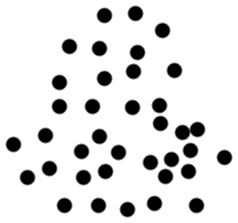
\includegraphics[scale=.25]{graphics/presentation/clusters2} 
        \end{figure}
        Query random points and fix the classifier to fit revealed data, but...\\
      \end{column}
      \begin{column}{5cm}
        \begin{figure}
          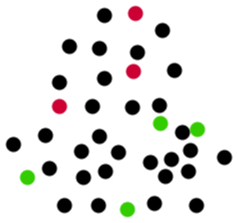
\includegraphics[scale=.5]{graphics/presentation/al1} 
        \end{figure}
      \end{column}
    \end{columns}
  \end{frame}
  \begin{frame}
    \frametitle{Naive active learning, cont.}
    \begin{columns}
      \begin{column}{5cm}
        \begin{figure}
          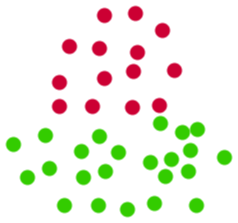
\includegraphics[scale=.25]{graphics/presentation/al1a} 
        \end{figure}
        ...it is not good in general.\\
      \end{column}
      \begin{column}{5cm}
        \begin{figure}
          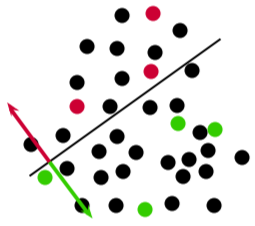
\includegraphics[scale=.5]{graphics/presentation/al1b} 
        \end{figure}
      \end{column}
    \end{columns}
  \end{frame}

  \begin{frame}
    \frametitle{Slightly better active learning---SVM inspired}
    \begin{columns}
      \begin{column}{5cm}
        \begin{figure}
          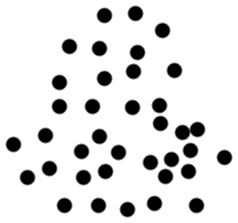
\includegraphics[scale=.25]{graphics/presentation/clusters2} 
        \end{figure}
        Once you have queried initial set of points, send to the oracle all exemplars that are placed in \emph{uncertainty zone}, but...\\
      \end{column}
      \begin{column}{5cm}
        \begin{figure}
          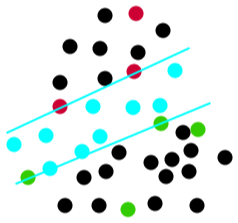
\includegraphics[scale=.5]{graphics/presentation/al1c} 
        \end{figure}
      \end{column}
    \end{columns}
  \end{frame}
  \begin{frame}
    \frametitle{Slightly better active learning---SVM inspired, cont.}
    \begin{columns}
      \begin{column}{5cm}
        \begin{figure}
          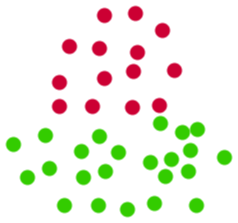
\includegraphics[scale=.25]{graphics/presentation/al1a} 
        \end{figure}
        ...it is inefficient---to many queries: $16$ which is about $45\%$.\\

        It performs really bad with fixed \emph{query budget}.
      \end{column}
      \begin{column}{5cm}
        \begin{figure}
          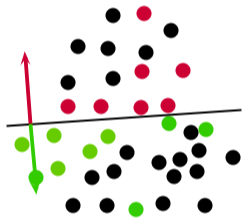
\includegraphics[scale=.5]{graphics/presentation/al1d} 
        \end{figure}
      \end{column}
    \end{columns}
  \end{frame}

  \begin{frame}
    \frametitle{``Perfect'' active learning}
    \begin{columns}
      \begin{column}{5.5cm}
        \begin{figure}
          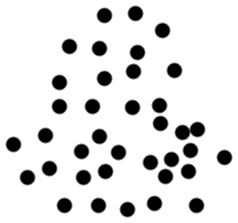
\includegraphics[scale=.25]{graphics/presentation/clusters2} 
        \end{figure}
        \begin{itemize}
          \item Identify a set of hypothesis---linear classifiers.
          \item According to some decision rule choose the best one and ask the oracle about the most informative point.
          \item Repeat above two steps until converged.
        \end{itemize}
      \end{column}
      \begin{column}{4.5cm}
        \begin{figure}
          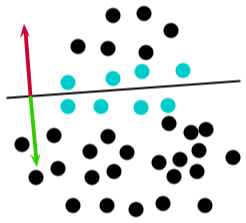
\includegraphics[scale=.5]{graphics/presentation/al1e} 
        \end{figure}
      \end{column}
    \end{columns}
  \end{frame}


\section{Is it really exploration vs. exploitation?} 
\subsection{Multi-armed bandits as a workhorse}
  \begin{frame}
  \frametitle{MAB}
  \begin{block}{Multi-armed bandits}
    \begin{itemize}
      \item MAB are sequential allocation problems.
      \item Agent at each stage has to take one out of $A$ available actions.
      \item Once the action is taken, the agent receives a feedback.
      \item To make the best possible choice at each stage the agent should utilise all the information and feedback gathered so far.
    \end{itemize}
  \end{block}
  \end{frame}
  \begin{frame}
  \frametitle{MAB, cont.}
  \begin{block}{Thompson Sampling policy}
    \begin{itemize}
      \item It is a Bayesian's approach.
      \item We model each action as a random variable with some underlying distribution, which parameters are unknown---our goal is to recover these parameters.
      \item By simulation we draw samples from our estimates of these distributions and take the action with the highest sample.
      \item By taking an action we receive a true sample which we can use(Bayes' theorem) to improve our estimates of parameters for this particular action.
    \end{itemize}
  \end{block}
  \end{frame}
  \begin{frame}
  \frametitle{MAB, cont.}
  Above set of rules provides us with right balance between exploration and exploitation.
  \begin{block}{Idea}
    \begin{center}
      Sample from the posterior.
    \end{center}
  \end{block}
  \end{frame}

  \begin{frame}
  \frametitle{Ingredients of AL}
  \begin{block}{Active learning}
    \begin{itemize}
      \item We have hypotheses(i.e.\ classifiers) which we want to test and choose the best one; we need a measure of how given hypothesis fits the data.
      \item We can query points, where each point sent to the oracle reveals some information about the state of our system---the true label of queried point; which we can model to be ours feedback signal.
    \end{itemize}
  \end{block}
  \end{frame}

  \begin{frame}
  \frametitle{Applying MAB to active learning}
  \begin{alertblock}{Sampling vector over the pool}
    $$
    p_n^t = p_{\text{min}} + (1-Np_{\text{min}}) 
    \frac{L(\hat{y}_n h(\mathbf{x}_n))}{\sum_{\mathbf{x}_n \in \mathscr{P}} L(\hat{y}_n h(\mathbf{x}_n))}
    $$
  \end{alertblock}
  \begin{block}{How to choose a point}
    \begin{itemize}
      \item According to current hypothesis we calculate a probability of each point being queried.
      \item The higher the loss suffered on given point the more probable it is that the point will be queried.
      \item We create a probability vector which underlies sampling distribution that we use to choose a point to query.
    \end{itemize}
  \end{block}
  \end{frame}
  \begin{frame}
  \frametitle{Applying MAB to active learning, cont.}
  \begin{block}{The feedback}
    \begin{itemize}
      \item For simplicity the points are allowed to be re-queried.
      \item The sampling vector approach guarantees non-sticking to single point.
      \item Once the point is chosen to be queried, it is sent to the oracle and its true label is revealed.
      \item Gained label improves both querying probability and hypothesis risk estimate.
    \end{itemize}
  \end{block}
  \end{frame}
  \begin{frame}
  \frametitle{Applying MAB to active learning, cont.}
  \begin{alertblock}{Risk of a hypothesis}
  $$
  \hat{L}_t(h) = \frac{1}{Nt} \sum_{n=1}^{N} \sum_{\tau = 1}^{t} 
\frac{Q^{\tau}_n}{p^{\tau}_n} L(y_n h(\mathbf{x}_n)) \text{~,}
  $$
  $$U(\hat{L}_t(h)) = \frac{ \sqrt{ \log(t) } }
                       { 10 }
                  \sqrt{ V^\prime_t }$$
  $$V^\prime_t = \left[
  \sum_{n = 1:N \text{~} \tau = 1:t} \left( \frac{Q^\tau_n}{p^\tau_n} L(y_n h(\mathbf{x}_n)) \right)^2
  -
  \left( \sum_{\mathscr{Q}_t} L(y_n h(\mathbf{x}_n)) \right)^2
\right]_+$$
  \end{alertblock}
  \end{frame}
  \begin{frame}
  \frametitle{Applying MAB to active learning, cont.}
  \begin{alertblock}{Risk of a hypothesis}
  $$
  \hat{L}_t(h) = \frac{1}{Nt} \sum_{n=1}^{N} \sum_{\tau = 1}^{t} 
\frac{Q^{\tau}_n}{p^{\tau}_n} L(y_n h(\mathbf{x}_n)) \text{~,}
  $$
  \end{alertblock}
  \begin{exampleblock}{How it works}
    \begin{itemize}
      \item The risk is \emph{inversely proportional} to the number of points and current time.
      \item We are effectively summing over all queried points up to time $t$.
      \item We sum loss of exemplar weighed by \emph{probability that given point should be queried at given time}.
      \item If probability of querying given point was small the loss on this particular point will count less towards hypothesis risk.
    \end{itemize}
  \end{exampleblock}
  \end{frame}
  \begin{frame}
  \frametitle{Applying MAB to active learning, cont.}
  \begin{block}{Why loss?}
    \begin{itemize}
      \item The further the point is from the classifier while being correctly classified the lower the loss is.
      \item On contrary, if it is far away and is miss-classified it will receive high loss.
      \item If the points are close to the classifier we are the most uncertain about them. Therefore, they have average contribution as the data may be noisy.
    \end{itemize}
  \end{block}
  \end{frame}
  \begin{frame}
  \frametitle{Applying MAB to active learning, cont.}
  \begin{alertblock}{Risk of a hypothesis}
  $$U(\hat{L}_t(h)) = \frac{ \sqrt{ \log(t) } }
                       { 10 }
                  \sqrt{ V^\prime_t }$$
  $$V^\prime_t = \left[
  \sum_{n = 1:N \text{~} \tau = 1:t} \left( \frac{Q^\tau_n}{p^\tau_n} L(y_n h(\mathbf{x}_n)) \right)^2
  -
  \left( \sum_{\mathscr{Q}_t} L(y_n h(\mathbf{x}_n)) \right)^2
\right]_+$$
  \end{alertblock}
  \begin{block}{How uncertain we are about the risk estimate}
    \begin{itemize}
      \item As $\log$ function is slowly increasing the uncertainty with time.
      \item It is similar to sample or population variance estimate.
      \item We make sure it is non-negative.
    \end{itemize}
  \end{block}
  \end{frame}
  \begin{frame}
  \frametitle{Proposed solution}
    \begin{exampleblock}{MAB-AL}
      \begin{enumerate}
        \item Chose hypothesis to test.
        \item Calculate sampling vector over the pool and choose a point to query; send the point to the oracle.
        \item Utilising queried points calculate risk and uncertainty of the risk for each hypothesis.
        \item Simulate normal distribution with the above parameters for each hypothesis and take a sample from each.
        \item Repeat above steps, with newly chosen hypothesis; loop until \emph{query budget} is exhausted.
      \end{enumerate}
    \end{exampleblock}
  \end{frame}


\subsection{The experiment}
  \begin{frame}
  \frametitle{The dataset}
    \begin{figure}
      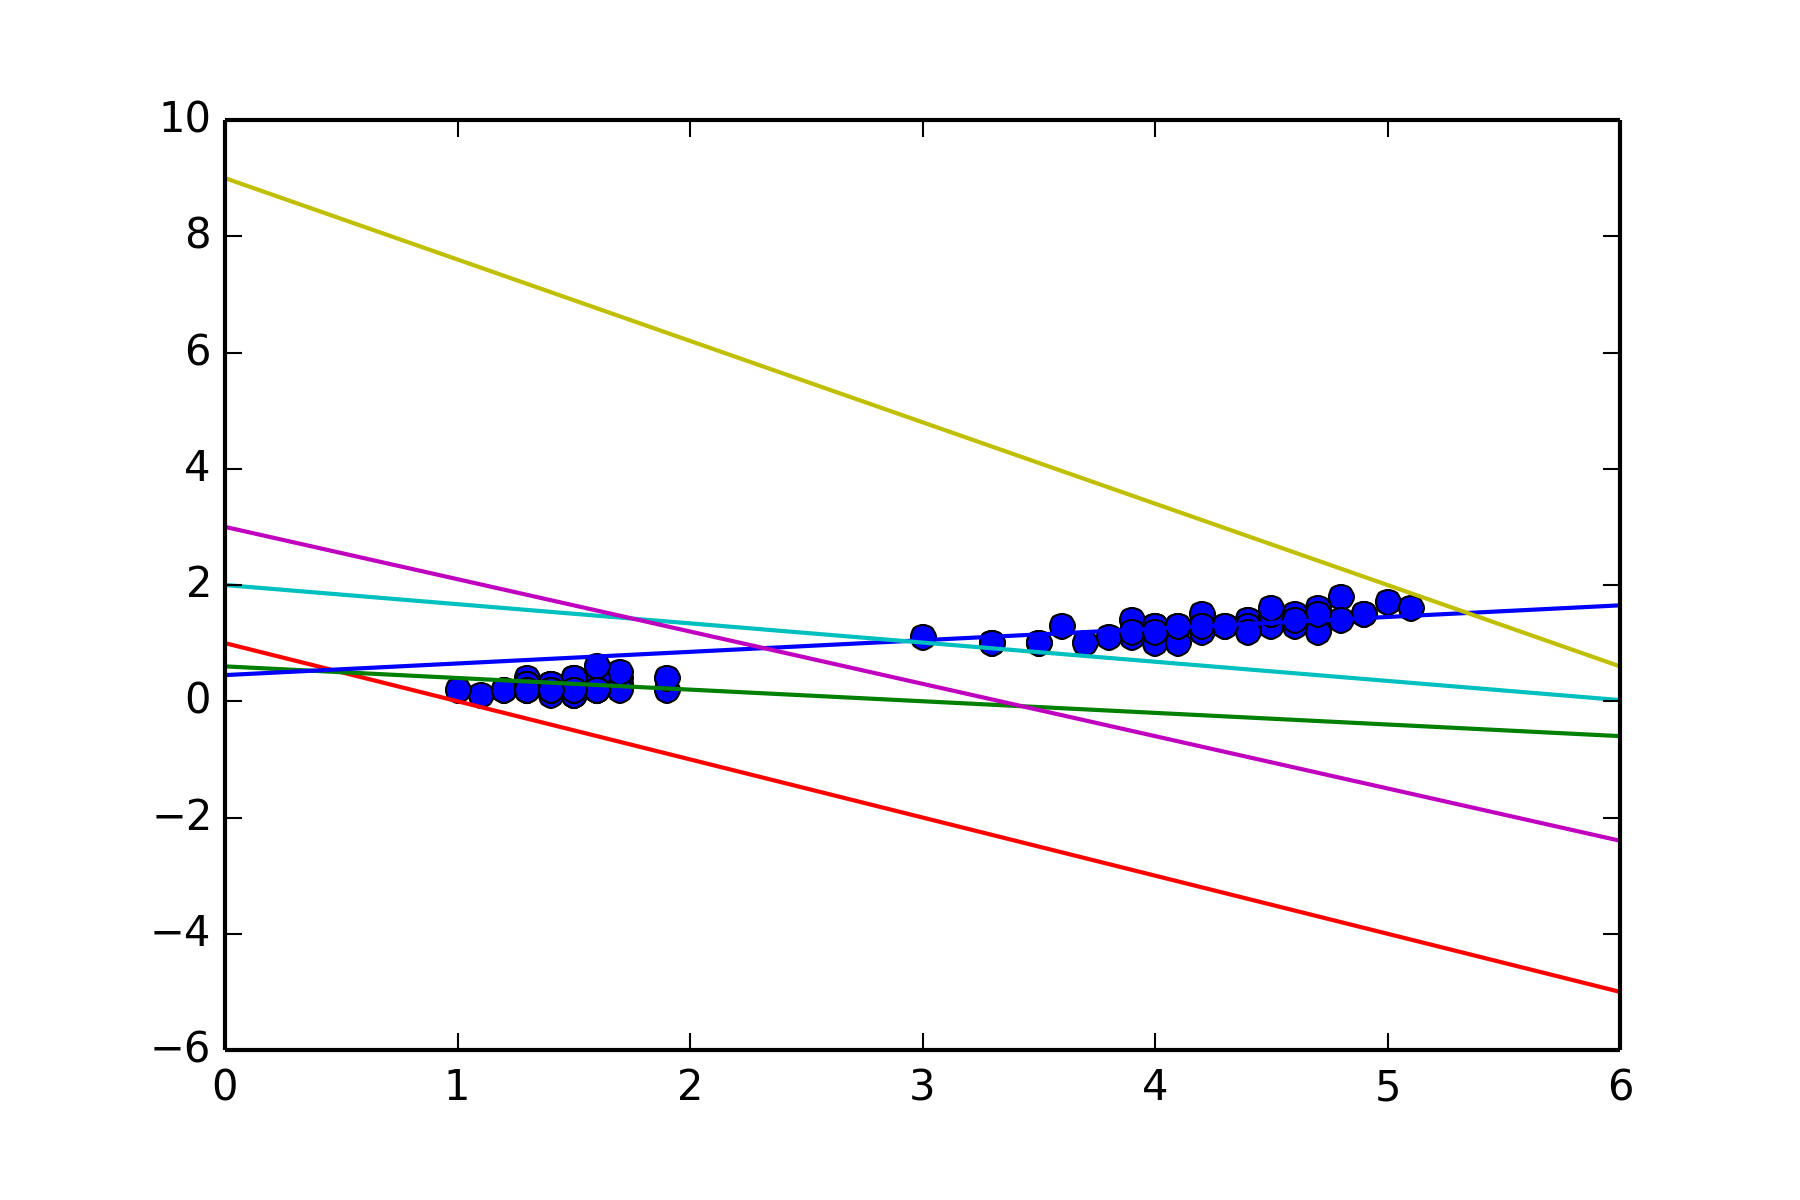
\includegraphics[scale=.7]{graphics/gypothesis} 
    \end{figure}
  \end{frame}
  \begin{frame}
  \frametitle{Arriving at optimal classifier}
    \begin{figure}
      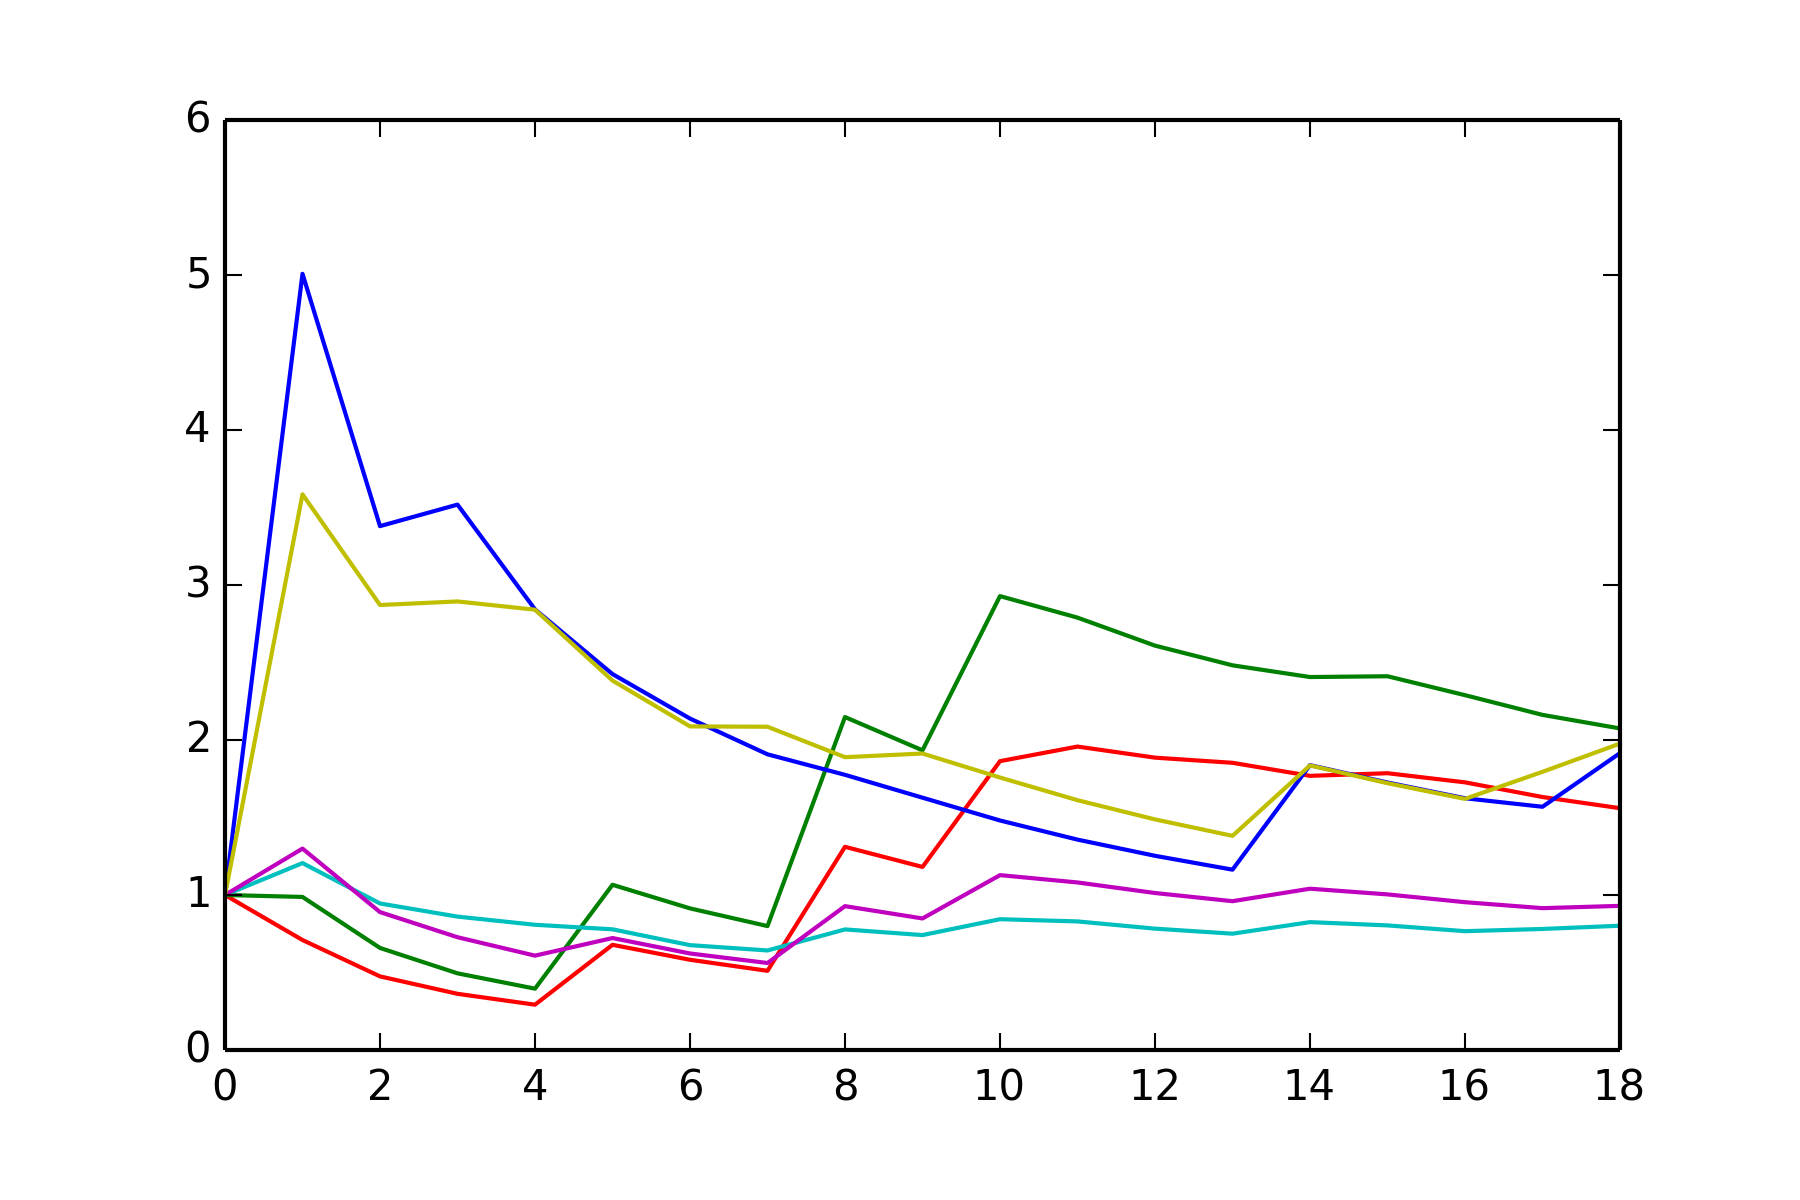
\includegraphics[scale=.7]{graphics/convergence15} 
    \end{figure}
  \end{frame}

  \begin{frame}
  \frametitle{Q\&A}
    \begin{columns}
      \begin{column}{5cm}
        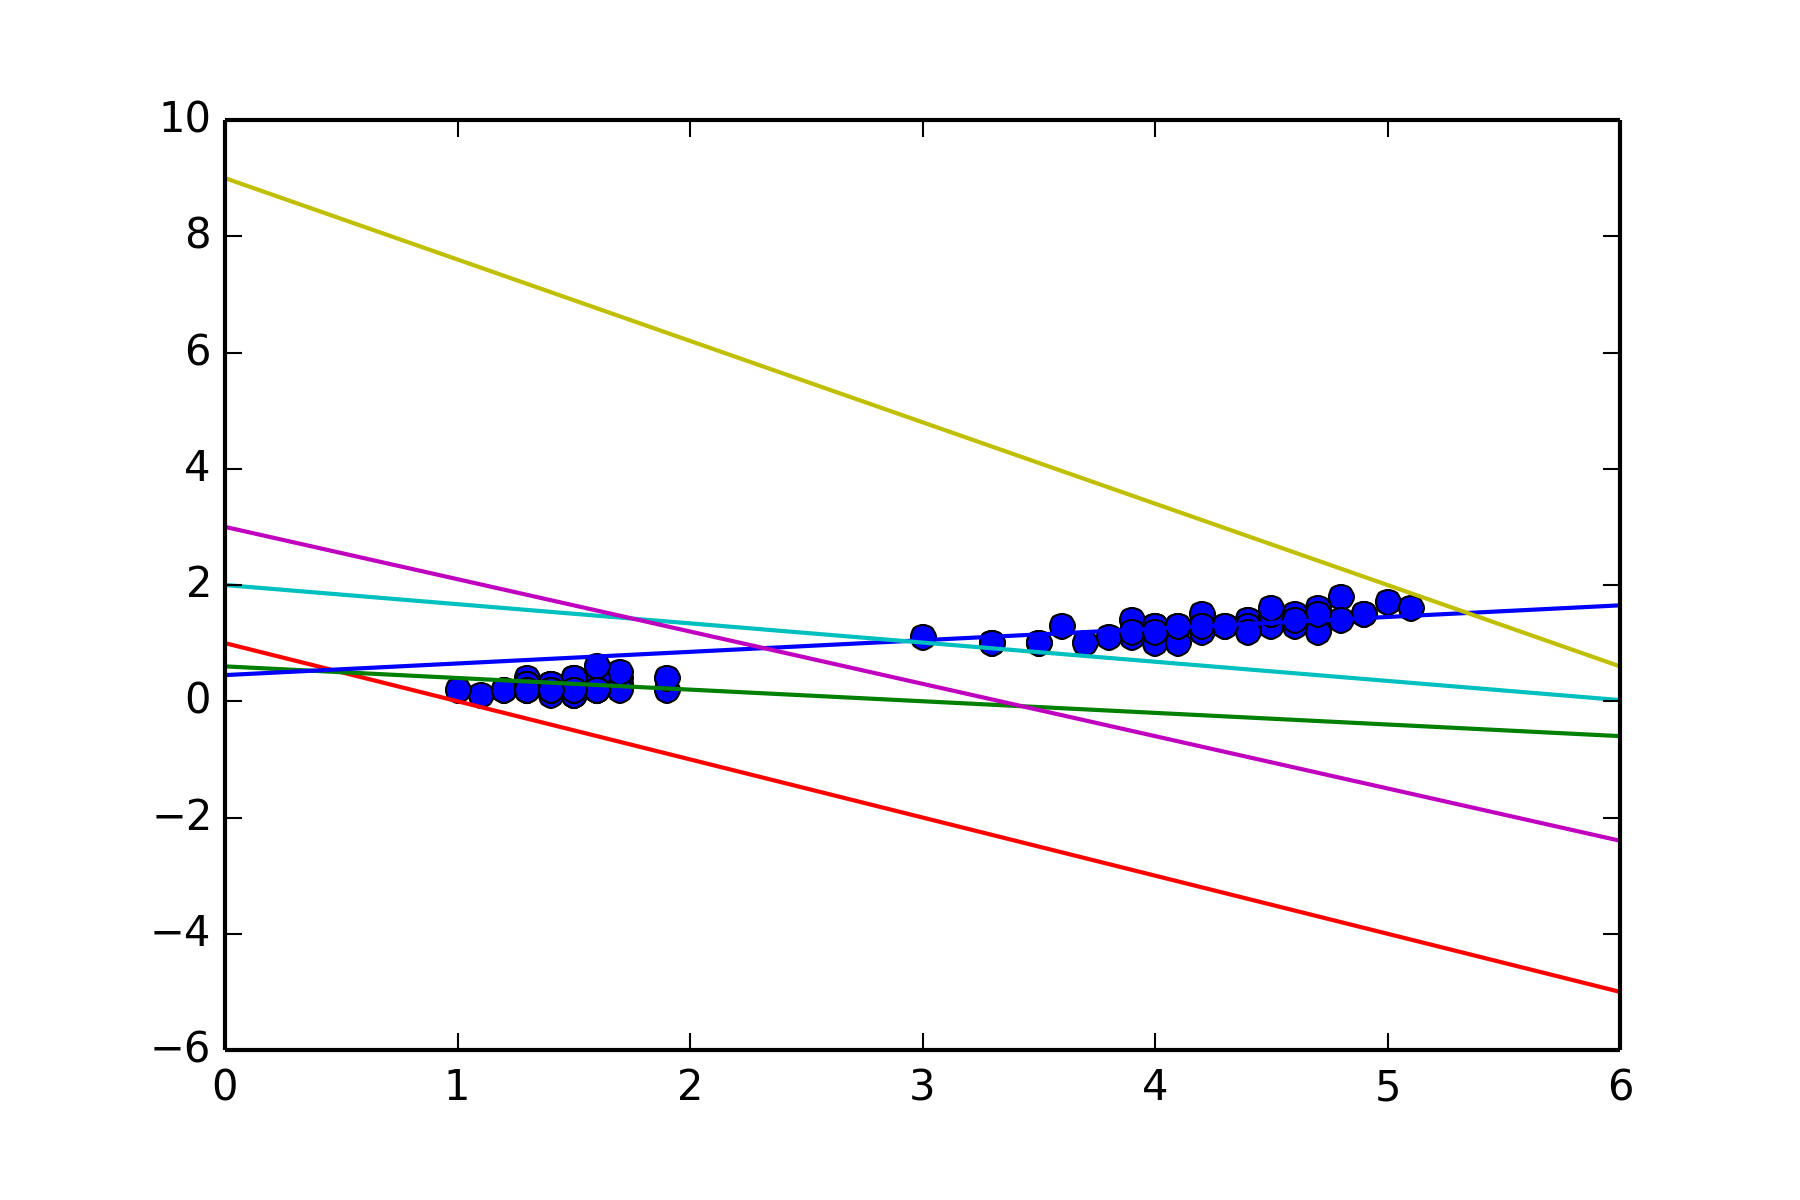
\includegraphics[scale=.4]{graphics/gypothesis} 
      \end{column}
      \begin{column}{5cm}
        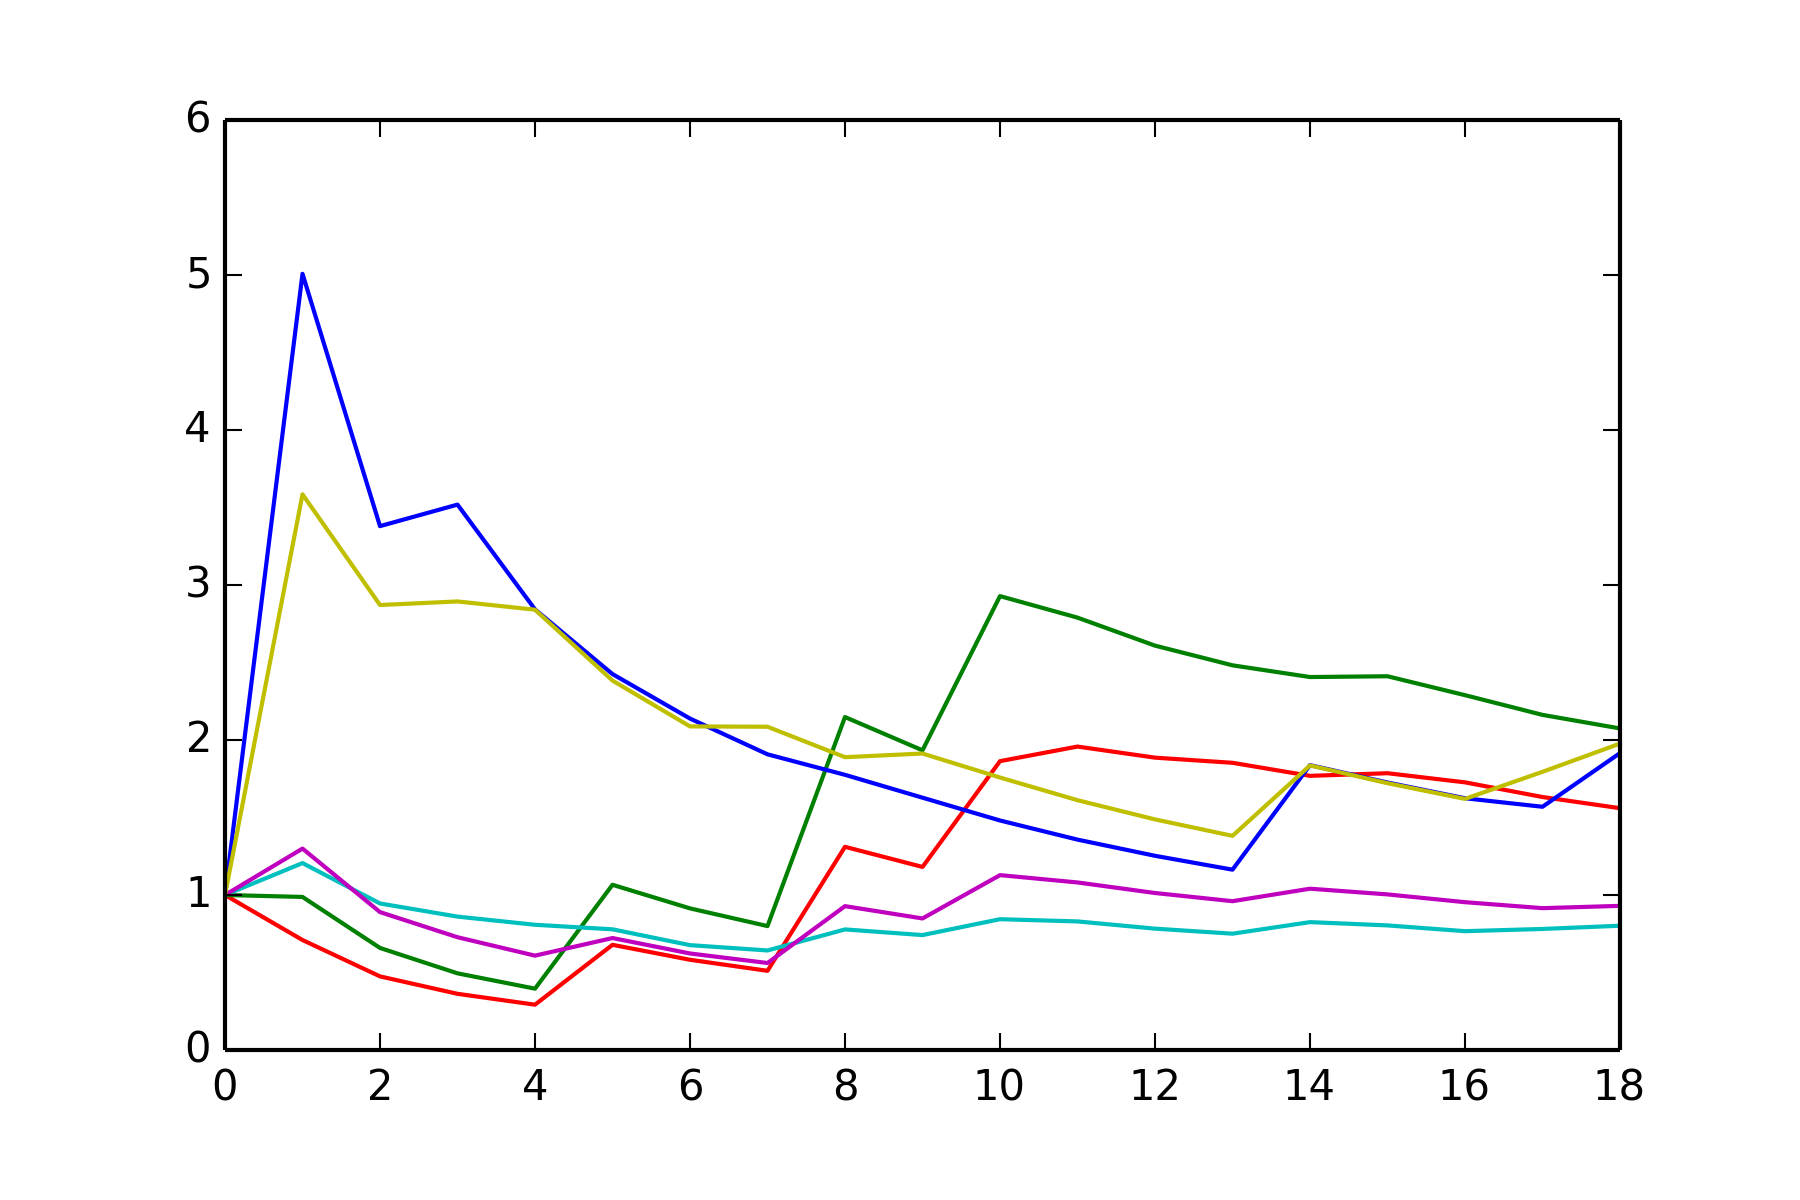
\includegraphics[scale=.4]{graphics/convergence15} 
      \end{column}
    \end{columns}
  \end{frame}

\end{document}

%%%%%%%%%%%%%%%%%%%%%%%%%%%%%%%%%%%%%%%%%%%%%%%%%%%%%%%%%%%%%%%%%%%%%%%%%%%%%%%%
% \begin{block}{title of the bloc}
% bloc text
% \end{block}
%
% \begin{exampleblock}{title of the bloc}
% bloc text
% \end{exampleblock}
%
% \begin{alertblock}{title of the bloc}
% bloc text
% \end{alertblock}
% 
% 
% \pause 
% 
% \begin{itemize}
% \item<1-> subject 1
% \item<3-> subject 2
% \item<5-> subject 3
% \end{itemize}
% 
% 
% \begin{overprint}
% \includegraphics<2>{PIC1}
% \includegraphics<4>{PIC2}
% \includegraphics<6>{PIC3}
% \end{overprint}
%%%%%%%%%%%%%%%%%%%%%%%%%%%%%%%%%%%%%%%%%%%%%%%%%%%%%%%%%%%%%%%%%%%%%%%%%%%%%%%%
